\section{Background}
\label{Related Work}


This section begins with a description of the Sunlight Taihu Light architecture. Several parallel read mapping approaches are then presented,
before we focus on the seed-and-extend approach

\subsection{Sunway Taihu Light Architecture}
\label{Sunway Taihu Light}

The Sunway Taihu Light has been manufactured by the National Research
Center of Parallel Computer Engineering \& Technology of the
People's Republic of China and is located at the Wuxi Supercomputing
Center. It provides a theoretical peak performance of 125 PFlop/s and
an effective performance-to-power ratio of over 6 GFlop/s per watt. It
consists of 40,960 nodes with 1.4 PB attached memory. The
interconnection network provides roughly 70 TB/s bisection bandwidth
and 12 GB/s point-to-point communication bandwidth.

\begin{figure}[!htb]
  \begin{center}
    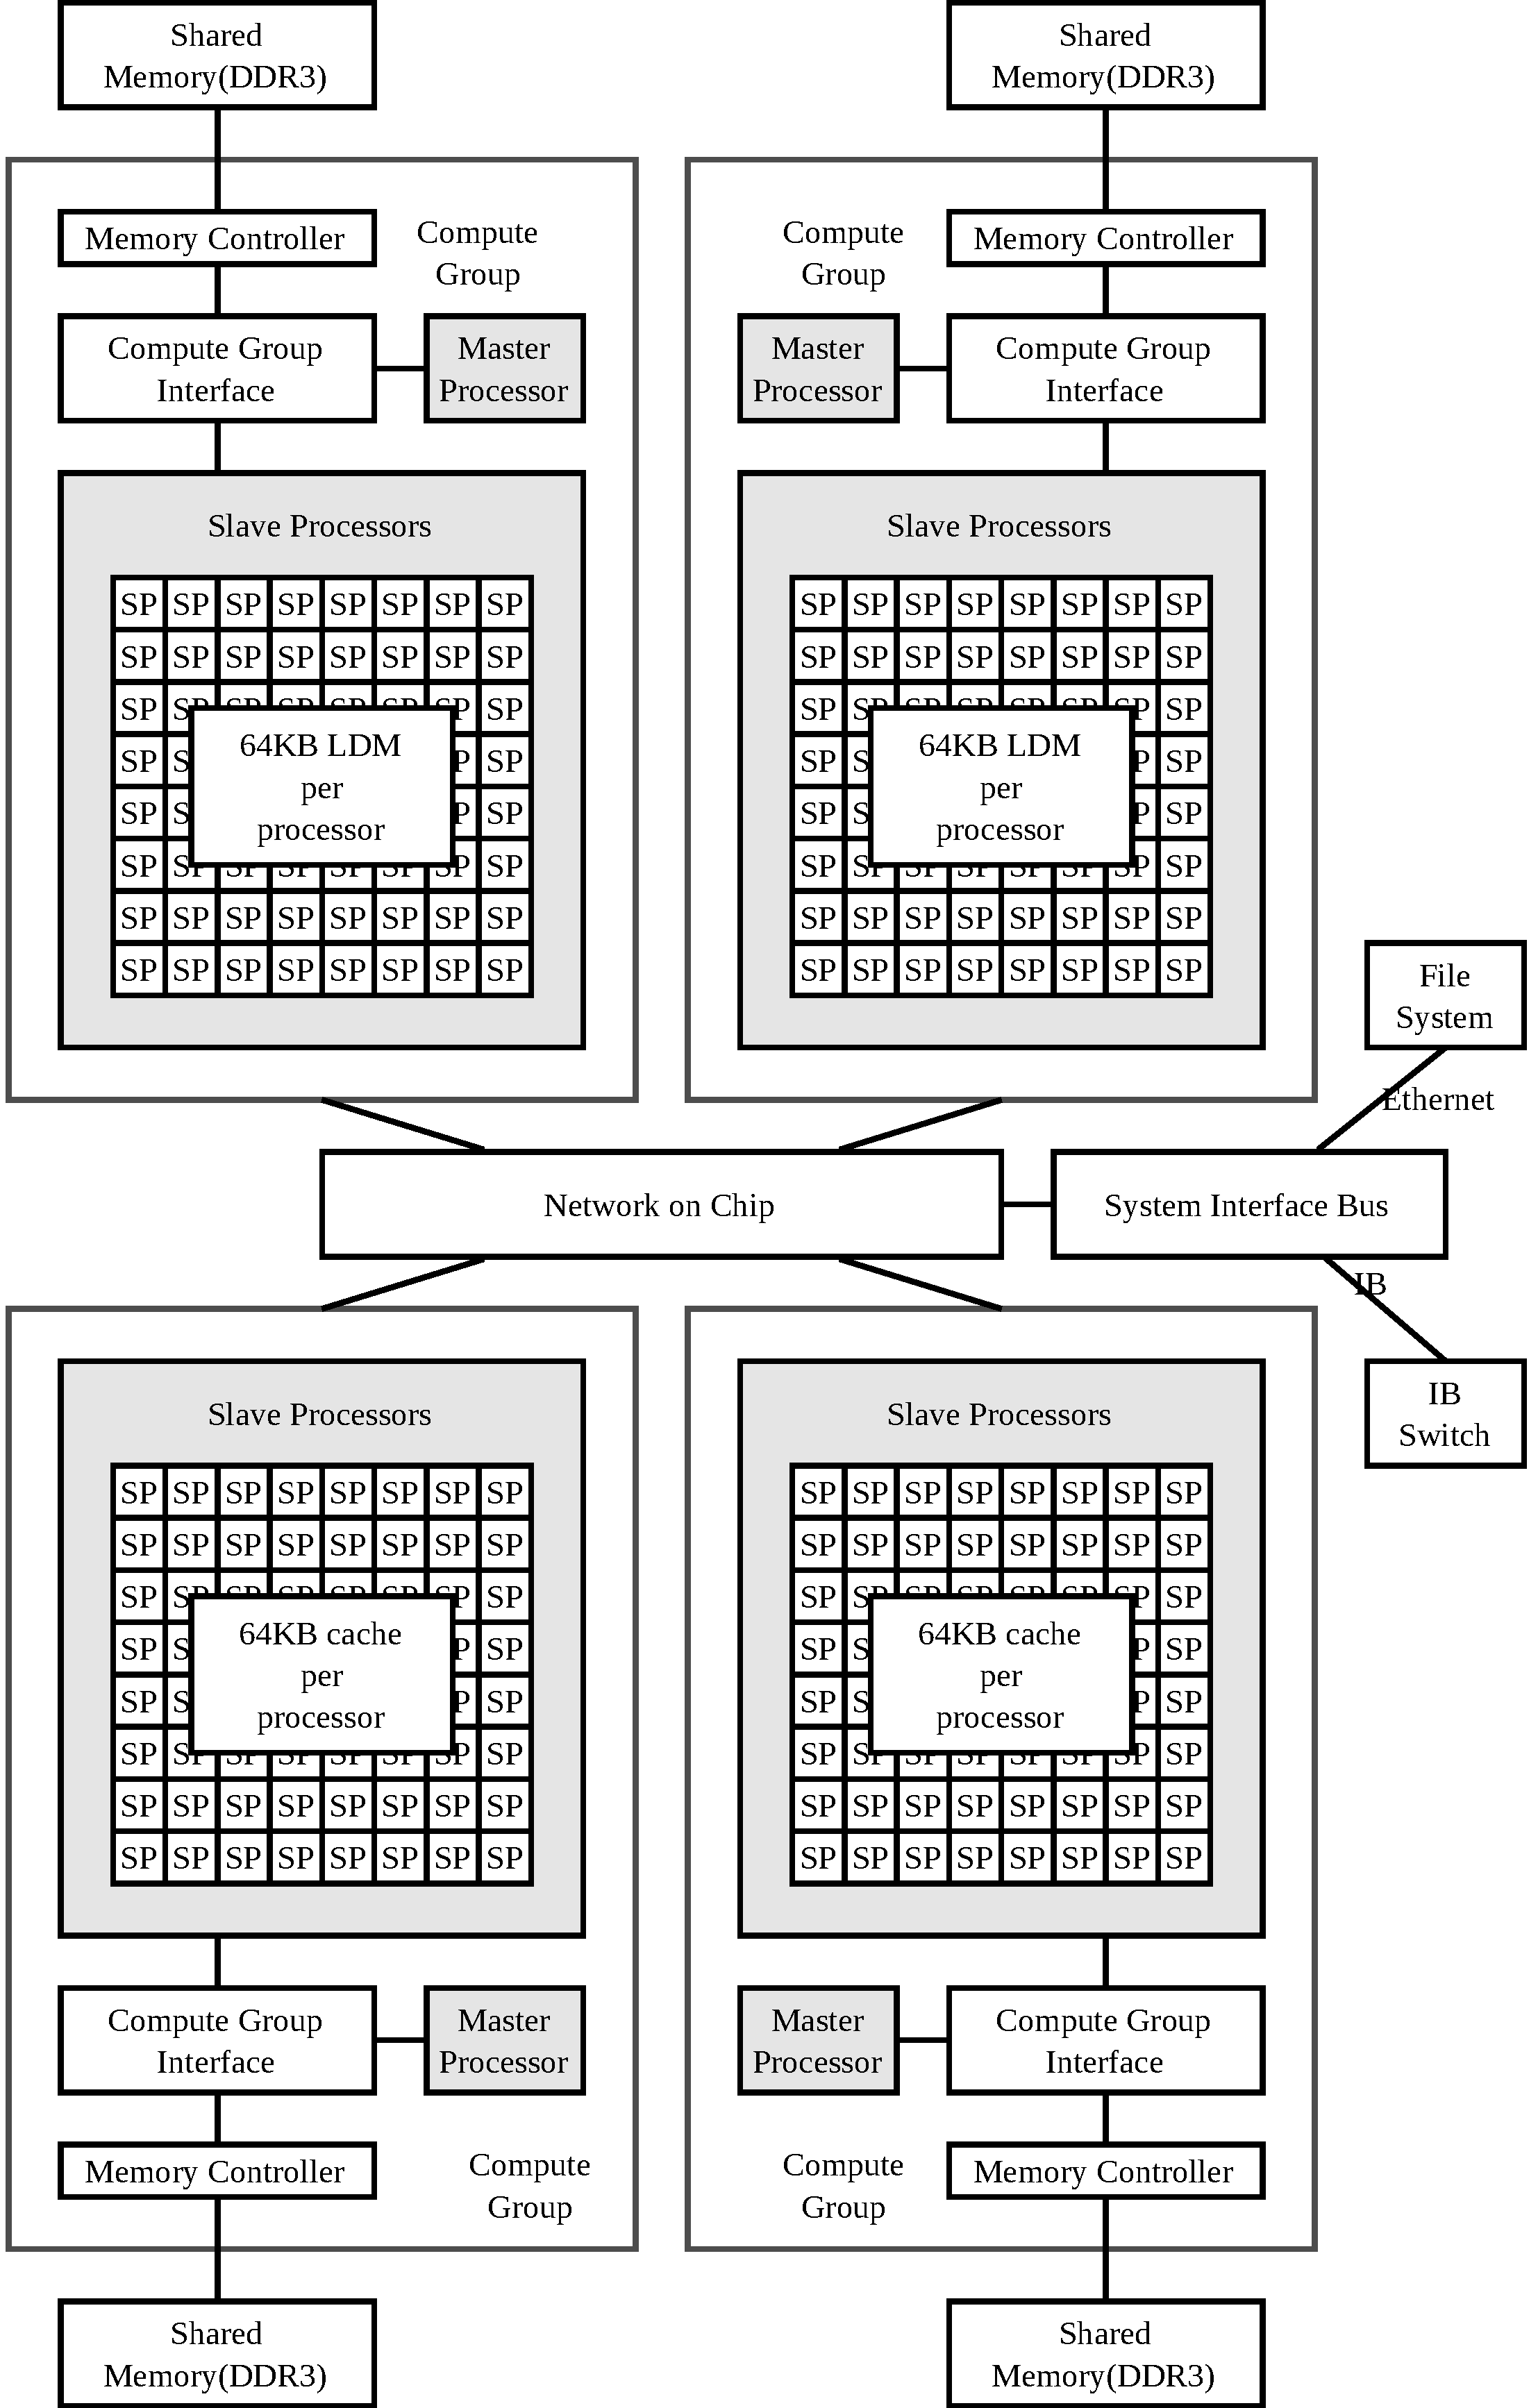
\includegraphics[width=\linewidth]{figures/SW26010}
    \caption{Architecture of the SW26010 processor, which is
      partitioned into four CGs.}
    \label{fig:SW26010}
  \end{center}
\end{figure}

Each node is equipped with a single SW26010 processor that is
subdivided into four CGs. A CG is the basic
unit that can be addressed by the job scheduling system. Each CG
consists of a single {\em master processor} (MP), 64 {\em slave
  processors} (SPs), and 8 GB of attached DDR3 shared memory. All
%Comment - slave is being replaced by worker  in much of the lit
nodes can access a shared network file system for loading and storing
data. The operating system is a customized Linux flavor running on the
MP.  Users may manually launch threads on the SPs in order to
parallelize compute-heavy portions of their code. Both the MP and 64
SPs support ShenWei's RISC basic instruction set, which provides
scalar and SIMD operations. Moreover, reduction primitives can be
called exclusively on the MP, while the SPs exhibit specialized
intrinsics for high-precision integer arithmetic. The 8 GB attached
shared memory can be accessed by both the MP and the 64 SPs via a
memory controller with a shared bandwidth of approximately 136
GB/s. The MP has its own cache (L1 and L2), and each SP can access 64
KB of fast {\em local device memory} (LDM). Data residing in shared
memory can be written to LDM by using DMA intrinsics and subsequently
communicated via a broadcast to the LDM of other
SPs. Figure~\ref{fig:SW26010} shows the hardware layout.

ShenWei's SIMD instruction set features 256-bit-wide vector types and
a set of corresponding intrinsics provided by the \emph{ShenWei 5
  Compiler Collection}.  The MPI library (Sunway MPI) is a derivative
of the MPICH implementation and is compliant with the MPI-3 standard.
Basic threading capabilities for the SPs are provided by the
\emph{athread} library.

\subsection{Related Work}

We are not the first to parallelize read mapping on a compute
cluster. Among the earliest tools are pBWA \cite{pbwa} and pMap
\cite{pmap}; pBWA is an MPI implementation of Version 0.5.9 of the BWA
aligner, whereas pMap provides an MPI-based framework for the concurrent
execution of popular aligners such as BWA \cite{bwa} and Bowtie
\cite{bowtie}. Other implementations exploit MapReduce frameworks, for
example, the Hadoop-based SEAL \cite{seal} and BigBWA \cite{bigbwa}
tools and the Spark-based SparkBWA suite \cite{sparkBWA}, in order to
guarantee fault tolerance. Unfortunately, all these approaches suffer
from insufficient scalability when executed on hundreds of nodes. The
metaframework parSRA \cite{parSRA} is designed for read mappers
written in UPC++.  It combines dynamic scheduling and a virtual file
system layer for read distribution to overcome the limitations imposed
by pMap and MapReduce-based approaches.
CUSHAW3-UPC++ \cite{cushaw3upc}
and merAligner \cite{merAligner}
are other PGAS-based short-read
aligners written in UPC; both demonstrate good scalability. Although
pMap and parSRA allow for the execution of single-node GPU aligners
such as nvBowtie \cite{nvBio}, none of the cited tools is explicitly
designed for heterogeneous clusters consisting of thousands of
many-core processors. Furthermore, all previous approaches target
traditional hardware architectures.

To the best of our knowledge, S-Aligner is the first attempt to
implement a fully scalable read mapper specifically designed to fit
the characteristics of Sunway Taihu Light. Previous algorithms mapped
onto this novel supercomputer have focused mainly on application
domains outside bioinformatics, such as Earth system modeling, ocean
surface wave modeling, atomistic simulation, and phase-field
simulation \cite{sunway}.

\subsection{Seed-and-Extend Approach}

Consider a set of reads ${\cal R}$, a reference genome $G$, and an
error threshold $e$. The read mapping problem can be defined as
follows: Find all substrings $g$ of $G$ that are within edit distance
$e$ to some read $R \in {\cal R}$. We call such occurrences $g$ in $G$
{\em matches}.

This problem can be solved by a classical {\em dynamic programming}
approach that calculates the semi-global alignment between each
$R \in {\cal R}$ and $G$. Unfortunately, each alignment results in a
time complexity proportional to the product of the sequences' lengths,
which renders intractable the alignment of a large number of short
reads to a reference genome a few billion letters long.  In order to
address this problem, most state-of-the-art solutions \cite{Reinert}
employ the {\em seed-and-extend} approach, which follows a three-stage
pipeline.

\begin{description}

\item{Stage 1: Filtration.} This stage identifies promising candidate
  regions (called {\em seeds}) for each read in $G$. A popular
  strategy in order to discard large regions of $G$ is based on the
  fact that if a read $R \in {\cal R}$ is divided into $e+1$
  non-overlapping $q$-grams (substrings of length $q = \lfloor \lvert
  R\rvert\ /(e+1) \rfloor$), then (according to the pigeonhole
  principle) at least one of them occurs exactly in a match. Such
  occurrences can be identified quickly by looking them up in
  precomputed $q$-gram index data structure (also called the {\em
    reference genome index}), which stores all substrings of length
  $q$ of $G$.

\item{Stage 2. Verification.} This stage determines whether a seed can
  actually be extended to a full match within edit distance $e$. This
  requires the implementation of a {\em verification} algorithm in
  order to analyze the vicinity of each seed. Most mappers typically
  apply fast versions of DP-based algorithms for this step.

\item{Stage 3. Alignment.} This stage generates the base-pair-level
  alignment information of a read and its verified intervals in $G$.

\end{description}

Established all-mappers such as RazerS3 \cite{razers3} and mrFAST
\cite{mrfast} follow this pipeline. Our profiling of RazerS3 and
mrFAST using a typical benchmark data set including the human
reference HG19 and 1 million simulated Illumina reads (with a read
length of 100 bps) reveals that Stage 2 occupies 67\% and 93\% of the
overall runtime, respectively. These results show that a fast implementation
of Myers' bit-parallel algorithm for computing the edit distance
between a read and an interval is a crucial component when designing
efficient all-mappers.

Consider two strings $s$ and $s^\prime$ of length $n$ and $m$,
respectively. Their {\em edit distance} is the minimum number of point
mutations (i.e., insertions, deletions, or substitutions) required to
transform $s$ into $s^\prime$. It can be determined by relaxing the
cells of a cost matrix $C$ of size $(n+1) \times (m+1)$ according to
the recurrence relation shown in Equation~\ref{update_scheme}, where
$0 < i \le n$ , $0 < j \le m$, and the {\em characteristic function}
$\chi (x \ne y)$ is 1 if $x \ne y$, and 0 otherwise. Initial
conditions are set to $C[i,0] = i$, $C[0,j] = j$, and $C[0,0] = 0$.

\begin{align}
  \label{update_scheme} 
  C[i,j]=\min \begin{cases} C[i-1,j-1]+\chi(s_{i-1} \neq s'_{j-1})\\
    C[i-1,j]+1 \\
    C[i,j-1]+1
  \end{cases}
\end{align}

Myers proposed a bit-vector algorithm \cite{myers} that exploits bit
parallelism by encoding the differences (deltas) between adjacent rows
and columns in the cost matrix $C$, as defined in
Equation~\ref{delta_update}, where $\varDelta h_{i,j}$, $\varDelta
v_{i,j}$, and $\varDelta d_{i,j}$ are the discrete derivatives of
$C[i, j]$ in the horizontal, vertical, and diagonal direction,
respectively.

\begin{align} \label{delta_update}
  \varDelta v_{i,j}&=C[i,j]-C[i-1,j]   &&\in \{0, \pm1\} \nonumber\\
  \varDelta h_{i,j}&=C[i,j]-C[i,j-1]   &&\in \{0, \pm1\} \\
  \varDelta d_{i,j}&=C[i,j]-C[i-1,j-1] &&\in \{0, +1\}   \nonumber
\end{align}

Note that the absolute values in Equation~\ref{delta_update} are
either 0 or 1. Thus, we can encode the relatively small state space
with the help of five vectors using one-hot
encoding. Figure~\ref{BitDP} shows an example of the encoding of the
vertical derivative $\varDelta v$ and its associated one-hot
representations $V^+$ and $V^-$.  With this bit-vector representation
the cell updates can be rewritten in terms of logical operations, as
shown in Equation~\ref{one-hot-myers}:

\begin{alignat}{100}
  \label{one-hot-myers}
  H^-_{i, j} &= \chi(\varDelta h_{i, j} &&= -1)            &&= V^+_{i, j-1} &&\land D^0_{i, j} \nonumber\\
  V^-_{i, j} &= \chi(\varDelta v_{i, j} &&= -1)            &&= H^+_{i-1, j} &&\land D^0_{i, j} \nonumber\\
  H^+_{i, j} &= \chi(\varDelta h_{i, j} &&= +1)            &&= V^-_{i, j-1} &&\lor \lnot(V^+_{i, j-1} \,\lor D^0_{i, j}) \\
  V^+_{i, j} &= \chi(\varDelta v_{i, j} &&= +1)            &&= H^-_{i-1, j} &&\lor \lnot(H^+_{i-1, j}   \lor D^0_{i, j}) \nonumber\\
  D^0_{i,j}  &= \chi(\varDelta d_{i, j} &&= \phantom{+}0)  &&= V^-_{i, j-1} &&\lor H^-_{i-1, j} \lor \chi(s_{i-1} = s'_{j-1}) \nonumber 
\end{alignat}

\begin{figure}[!htb]
  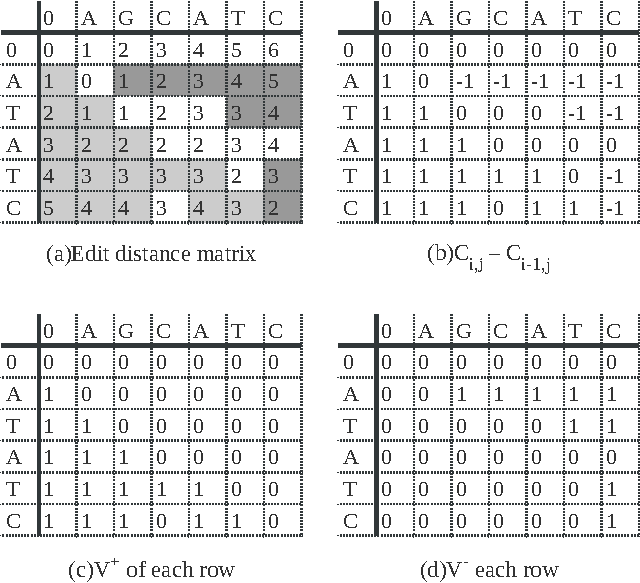
\includegraphics[width=1\linewidth]{figures/BitDP}
  \caption{Relations between the original matrix, $\varDelta v$,
    $V^+$, and $V^-$.  Here (a) shows the original score matrix;
    light-shaded cells indicate $\varDelta v_{i,j}=+1$ while heavily
    shaded cells correspond to $\varDelta v_{i,j}=-1$. The vertical
    derivative $\varDelta v$ shown in (b) is subsequently one-hot
    encoded by the bit vectors $V^+$ and $V^-$ in (c) and (d),
    respectively.}
  \label{BitDP}
\end{figure}
